\scanpage{10}
\mspage{3}
% Archive foliation: 9, upper left.
On suppose

(Hot 2) $\forall\ f:A\longrightarrow B$ dans $\mathrm{Cat}$, le foncteur
\deleted{$f^*:\unsure{\mathcal H(A)}$}
\[
f_{\mathcal H}^{*}:\mathcal H(B)\longrightarrow\mathcal H(A)
\]
a un \uline{adjoint à gauche}
\[
f_!^{\mathcal H}:\mathcal H(B)\longrightarrow\mathcal H(A)
\]
de sorte que $\mathcal H(A)$ devient aussi \uline{covariant} en
$A$.
Il faut faire Attention, s'il ne faudrait pas
se borner ici aux $f$ \uline{cofibrants}.
\margin{\uline{voir}}

Si $B=\Delta_0$, on trouve
\[
\mathcal H(A)\longrightarrow\mathrm{Hot}_{\mathcal H}
\]
\margin{où $\pi_A:A\longrightarrow\Delta_0$ la projection}
\margin{$(\pi_A)_!$}
noté $\int_A$, et appelé foncteur intégration
jouant le rôle \unsure{de un|d'un} $\underset{A}{\underset{\longrightarrow}{\lim}}$.

On en a donc, par transitivité
\[
\int_A\mathcal X=\int_B f_!(\mathcal X
\]
\[
f:A\longrightarrow B.
\]
\margin{NB L'existence des $f_!$ implique l'existence
des sommes dans les $\mathcal H(A)$, $\unsure{\leftarrow|<}$,
\deleted{$\unsure{f}$} \unsure{Bien sûr} les $f_!$ y \unsure{commutent}.}
\margin{\figure{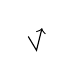
\begin{tikzpicture}[scale=.35]\draw[->] (0,.5)--(.3,0)--(.5,.8);\end{tikzpicture}}}

\textcircled{3} Opérations $\prod_A$ de cointégration,
\margin{\textcircled{Hot 3}}
par des $f_*^{\mathcal H}$ adjoints à droite des $f_{\mathcal H}^{*}$.
